\documentclass[conference]{IEEEtran}
\IEEEoverridecommandlockouts
% The preceding line is only needed to identify funding in the first footnote. If that is unneeded, please comment it out.


\usepackage{multirow}
\usepackage{makecell}
\usepackage{color}
\usepackage{cite}
\usepackage{amsmath,amssymb,amsfonts}
\usepackage[Alg.]{algorithm}
\usepackage[noend]{algpseudocode}
\usepackage{float} 
\usepackage{graphicx}
\usepackage{subfigure}
\usepackage{textcomp}
\usepackage{xcolor}
\usepackage{url}
\usepackage{cite}

\def\BibTeX{{\rm B\kern-.05em{\sc i\kern-.025em b}\kern-.08em
    T\kern-.1667em\lower.7ex\hbox{E}\kern-.125emX}}
\begin{document}

\title{Applying the Restart Policy to Hardware Model Checking Boosts Bug-Finding
%{\footnotesize \textsuperscript{*}Note: Sub-titles are not captured in Xplore and
%should not be used}
%\thanks{Identify applicable funding agency here. If none, delete this.}
}

\iffalse
\author{\IEEEauthorblockN{1\textsuperscript{st} Given Name Surname}
\IEEEauthorblockA{\textit{dept. name of organization (of Aff.)} \\
\textit{name of organization (of Aff.)}\\
City, Country \\
email address or ORCID}
\and
\IEEEauthorblockN{2\textsuperscript{nd} Given Name Surname}
\IEEEauthorblockA{\textit{dept. name of organization (of Aff.)} \\
\textit{name of organization (of Aff.)}\\
City, Country \\
email address or ORCID}
\and
\IEEEauthorblockN{3\textsuperscript{rd} Given Name Surname}
\IEEEauthorblockA{\textit{dept. name of organization (of Aff.)} \\
\textit{name of organization (of Aff.)}\\
City, Country \\
email address or ORCID}
\and
\IEEEauthorblockN{4\textsuperscript{th} Given Name Surname}
\IEEEauthorblockA{\textit{dept. name of organization (of Aff.)} \\
\textit{name of organization (of Aff.)}\\
City, Country \\
email address or ORCID}
\and
\IEEEauthorblockN{5\textsuperscript{th} Given Name Surname}
\IEEEauthorblockA{\textit{dept. name of organization (of Aff.)} \\
\textit{name of organization (of Aff.)}\\
City, Country \\
email address or ORCID}
\and
\IEEEauthorblockN{6\textsuperscript{th} Given Name Surname}
\IEEEauthorblockA{\textit{dept. name of organization (of Aff.)} \\
\textit{name of organization (of Aff.)}\\
City, Country \\
email address or ORCID}
}
\fi

\maketitle

\begin{abstract}
Model checking is an efficient technique for verification of hardware designs. However, its performance, particularly on bug-finding, needs to be improved to meet the industrial requirement. In this paper, we focus on improving CAR, a recently proposed model checking technique, by applying simple restart policies to the algorithm. Our results show that, out of the 749 industrial instances,  CAR with different restart policies is able to find 17 instances that the state-of-the-art technique BMC can not find, and solve more than 12 instances than its previous version. The new algorithm succeeds to contribute to the current model-checking portfolio in practice.  

\iffalse
In recent years, SAT-based model checking have been proven to be the powerful techniques for verification of  safety-critical systems such as the hardware designs. In particular, Bounded Model Checking (BMC) is considered as the most efficient verification technique for the bug detection, or bug-finding. Recently, a new method of model checking, which is named CAR (Complementary Approximate Reachability), has been shown the efficiency on bug-finding because of its ability to complement BMC by solving instances that cannot be solved by BMC within the same time and hardware sources. Nevertheless, CAR cannot detect as many bugs as BMC in current stage. In this paper, we present our results on applying the restart policy, which has been widely used in modern SAT solvers, to CAR, to obtain a better performance of bug-finding. Our results show that, out of the total 749 industrial instances, by invoking the restart policy with different parameters, CAR is able to find 17 instances that BMC can not find and solve more than 10 instances than the previous version, which yields a significant improvement on the bug-finding performance.
\fi
\end{abstract}

\begin{IEEEkeywords}
Model Checking, CAR, BMC, SAT, Bug-finding
\end{IEEEkeywords}

\section{Introduction}
In the hardware design community, model checking \cite{CGD99} has emerged as a popular technique for both bug-finding and correctness proof of hardware systems (circuits). Given a hardware design $M$ as the model and the formal specification (property) $P$, model checking checks whether $P$ holds for all behaviours of $M$. To achieve this goal, a model-checking algorithm explores the state space of $M$ by starting from the initial states to all their reachable states in $M$. Moreover, model-checking techniques terminate the exploration as soon as 1) a counterexample to represent the property violation is detected, or 2) the proof is accomplished that the initial states can never reach the states which violate the property $P$. If $P$ is a safe property, the length of the counterexample becomes finite. As a result, the safety model checking can be reduced to the reachability analysis problem \cite{KV99c}, and we focus on the safety model checking in this paper.  


Although model checking has been widely used in hardware verification, the performance improvement is still eagerly on demand to help solve more industrial instances. It is well known that no model-checking technique is the best one to dominate all others, and different algorithms perform differently for different benchmarks \cite{GR16}. Although invented in nearly three decades ago, Bounded Model Checking (BMC) \cite{BCCFZ99,BCCZ99} is still considered to be the most efficient technique for detecting bugs.  Meanwhile,  Interpolation Model Checking (IMC) \cite{McM03} and IC3 \cite{Bra11}, or Property Directed Reachability  (PDR) \cite{EMB11}, are shown more powerful to prove correctness. Therefore, a portfolio of model checking techniques is often maintained by the industry companies to solve different problems.

Recently, a new model-checking algorithm named Complementary Approximate Reachability (CAR) \cite{LZZPV17}, was proven to complement BMC on bug-findings and IC3/PDR on correctness proofs. That is, CAR is able to solve instances that BMC or IC3/PDR cannot solve within the given time and hardware sources. The achievement from CAR inspires us that, even relevant techniques have been deeply investigated for decades, there are possibilities to improve the model-checking performance such that it can be more useful for the industry. In this paper, we focus on CAR and present an improved search strategy inside the algorithm to gain a better bug-finding performance.  


CAR was inspired by IC3/PDR and the traditional reachability analysis \cite{LZZPV17}, which maintains an over-approximate state sequence for correctness proof and an under-approximate state sequence for bug-finding. CAR utilizes the depth-first search strategy to find new states that meet the constraints, which are used to refine the under-approximate state sequence, or if failed, collect the relevant  information to refine the over-approximate state sequence. The algorithm terminates as soon as either a \emph{bad} state is in the under-approximate sequence, which indicates a counterexample has been detected, or an \emph{invariant} has been computed based on the over-approximate sequence, which indicates the correctness proof has been asserted.  For more details see below. CAR can be performed in both forward and backward directions. Since evidences have shown Backward-CAR is better than Forward-CAR \cite{LDPRV18}, we follow the observation and focus on improving Backward-CAR. In the rest of the paper, all mentions of ``CAR'' represent Backward-CAR. 

Although CAR has been shown the advantage of detecting bugs for safety model checking and outperforms IC3/PDR on bug-finding, it cannot solve as many unsafe instances (those with bugs) as BMC in the current stage \cite{DLPVR19}. Looking into the state paths generated by CAR during the search, the observation comes up that, the depth-first strategy may lead the algorithm to a \emph{trap} for those unsafe cases unable to solve. As a result, to keep searching new states is almost impossible for the algorithm to locate the bad states but only wastes the computation sources. Such similar phenomenon occurs on solving the satisfiability of Boolean formulas (SAT) \cite{VWM15}, in which the search can also be in the trap if the order of variable assignments is not properly chosen. To tackle such issue, researchers propose a \emph{restart} policy such that the current search path is discarded and a new one can be selected to get rid of the trap \cite{Biere08}. Their experiments show that such simple strategy is very efficient to help speedup  SAT solving computation, particularly for those satisfiable instances. 

Inspired from the result achieved by applying the restart policy to modern SAT solvers \cite{Biere08}, we leverage the similar idea to enhance the performance of CAR on bug-finding. In our designation, the restart policy is invoked as soon as the size of new elements of the over-approximate state sequence in a single search, reaches the \emph{frequency} $k*t$ where $k$ is the length of the over-approximate sequence and $t$ is a given  \emph{threshold}, which can be dynamically updated based on a given \emph{growth rate} $gr$ during the search. That means, if the current threshold is $t$ and the growth rate is $gr$, the threshold will be updated to be $(t*gr)$ when the restart is invoked next time. Moreover, the search will be restarted next time as soon as the size of new elements of the over-approximate sequence reaches $(k*t*gr)$. As a result, the restart frequency depends on the threshold and the corresponding proportion to update it. Once the restart is triggered, CAR deletes all states information collected in the current search and start a new one immediately. 


We conduct a comprehensive experimental evaluation on  the 749 industrial instances from Hardware Model Checking Competition 2015 \cite{hwmcc15} and 2017 \cite{hwmcc17}. We implement our new algorithm based on the SimpleCAR model checker \cite{LDPRV18}\cite{simplecar}, and compare the bug-finding performance to the original CAR in SimpleCAR as well as the BMC algorithm that is implemented in the ABC model checker \cite{BM10}. The results show that, given the same time and hardware sources, our new algorithm can solve 18 more unsafe instances than BMC and 13 more than the original CAR, by feeding the restart policy with different frequencies. Although the new algorithm with a single configuration does not have a better performance than the original CAR, it does help increases the diversity to solve more instances, and therefore, increases the power of the current model-checking portfolio in the industry. 


\iffalse
Our algorithm Complementary Approximate Reachability(CAR), derived from traditional reachability analysis, is a SAT-based model checking technique that can run in two modes: forward-CAR and backward-CAR. As Backward-CAR has shown superior performance than forward-CAR in previous work, we focus on the backward-CAR and the word "CAR" will refer in particular to Backward-CAR in the following sections. The CAR algorithm maintains two sequences of abstract reachable state-sets, one is an under-approximate reachable state-sets origin from the initial states and the other is an over-approximate reachable state-sets which are generated from the bad states(the state-set violating the safety property P). 


Nowadays, a challenge in the field of hardware model checking is that the state space is too large compared to today's computing power. Due to the huge state space, a remarkably small part of the computation is used in the right place, most of the computation is just been used like looking for a needle in a haystack. A policy is needed to switch to another searching location when probably there will be no results in the current area. Previously, CAR algorithm sometimes gets stuck in a cyclical process that constantly forwarding and backtracking in certain state spaces. Inspired from the substantial effect of restart policy used in today’s clause learning SAT solvers, we apply a simple restart policy on the CAR algorithm to enhance its performance in bug-findings. We hold the opinion that the endless loop indicates it is hard to find a counterexample or a bug through this route(but not completely impossible) and the restart policy enables the algorithm to get out of the loop and then find another. 


We perform an extensive experiment based on a total of 749 industrial instances, and the results indicate that the restart policy can effectively expand the diversity of our hardware model checking algorithm: Complementary Approximate Reachability(Shorthand for the CAR). It seeks out 12 more new instances of counterexample. 

In this paper, we would like to take a step toward studying the effectiveness of applying restart policy on CAR with a view to motivating further work of designing an appropriate restart policy.
\fi

\section{PRELIMINARIES}

\subsection{Boolean transition system}

Modern SAT-based model checking techniques consider the \emph{Boolean transition system} as the model. A \textit{Boolean transition system} $Sys$ is a tuple $(V,I,T)$, where $V$ is a set of Boolean variables, and each state s of the system is in $2^{V}$, the set of truth assignments to variables in $V$. $I$ is the set of initial states. If we mark the copy of $V$ as $V^{'}$ to represent the set of primed variables, $T$ is the transition relation of the system over $V \cup V^{'}$. We say that state $s_{2}$ is a \textit{successor} of state $s_{1}$, iff $s_{1} \cup s^{'}_{2} \models T$, denoted $(s_{1},s_{2}) \in T$.


A finite state squence $s_{0},s_{1},......,s_{k}$ is called a path of length $k$, if each $(s_{i},s_{i+1})$ for $(0 \leq i \leq k-1)$ is in $T$. We say the state $t$ is reachable from state $p$ in (resp. within) $k$ steps, if there exists a finite path with length $k$ (resp. smaller than $k$) such that $s_{0} = p$ and $s_{k} = t$ are true. The set of all states that are reachable from the initial states $I$ is called the reachable states of $Sys$.
Given a safety property $P$ (represented as a Boolean formula) and Boolean transition system $Sys = (V,I,T)$, we say the system is \emph{safe} if $P$ holds for all the reachable states of $Sys$. Otherwise, the system is \emph{unsafe}. We call the state violating $P$ is a \emph{bad} state and use $\neg P$ to denote the set of all bad states. A path from an initial state in $I$ to one of the bad states in $\neg P$ is called a \emph{counterexample}.

Let $X \subseteq 2^{V}$ be a set of states in $Sys$. We define the relation $R(X)$ to be the set of successors of the states in $X$, i.e.,  $R(X) = \lbrace s^{'}|(s,s^{'}) \in T\, \textit{ for }s \in X \rbrace$. We define $R^{i}(X) = R(R^{i-1}(X))$ for $i > 1$. Similarly, we define $R^{-1}(X)$ as the set of predecessors of states in $X$ and $R^{-i}(X)$ analogously for $i > 1$.

We call a Boolean variable $a$ or its negation $\neg a$ as a \emph{literal}.
Let $L$ be a set of literals. A \emph{cube} is Boolean formula with the form of $\bigwedge l$ where $l\in L$. Analogously, a \emph{clause} is Boolean formula with the form of $\bigvee l$ where $l\in L$. It is not trivial to see that a state of $Sys$ is a cube.

\subsection{SAT calls with assumptions and unsatisfiable core}
The CAR algorithm frequently invokes the SAT calls whose inputs have the form of $A\wedge B$, where B is a CNF formula\footnote{The Boolean formula with the form of $\bigwedge c_i$ where each $c_i$ is a clause.} and A is a cube. We use the notation $SAT(A, B)$ to represent such SAT query and take $A$ as the \emph{assumptions} of the SAT solver. Although the result of $SAT(\emptyset,A \bigwedge B)$ is equivalent to that of $SAT(A,B)$, using the latter one is typically more flexible for incremental SAT calling, which is a very efficient mechanism to frequently invoke SAT solvers in practice.   
There are two different outcomes from an SAT solver when handling the query $SAT (A, B)$. If the result is \emph{satisfiable}, an assignment of the formula $A\wedge B$ is provided by the SAT solver. Otherwise, $A\wedge B$ is unsatisfiable and an Unsatisfiable Core (UC) $uc\subseteq A$, which is a subset of the assumptions $A$, can be returned by the SAT solver.

\iffalse
In the CAR algorithm, A is usually an explicit state and B is $T \bigwedge B_{i}$, where $T$ is the transition system of $Sys=(V,I,T)$ and $B_{i}$ is the \textit{i}-th level of B-sequence(will describe in below).

A SAT call like $\mathit{SAT}(A,B)$ will have two possible outcomes: 

1.satisfied, we will then use \textbf{get\_assignment()} to get a satisfying assignment to literals in A and B. 

2.unsatisfied, we will then use \textbf{get\_unsat\_core()} to get an unsatisfiable core c that $ c \subseteq A $ and $ c \bigwedge T $ is unsatisfiable.


In mathematical logic, given an unsatisfiable Boolean propositional formula in conjunctive normal form, like $\mathit{SAT}(A,B)$, if the outcome is unsatisfied, a subset of clauses whose conjunction is still unsatisfiable is called an unsatisfiable core of the original formula. In the CAR algorithm, the unsatisfiable core comes from the assumption which means it only contains some of the literals from the assumption. For example, given an unsatisfied SAT call $\mathit{SAT}(A,B)$, where A is a conjunction of literals $A=l_{1}\cap l_{2}\cap l_{3}\cap ...\cap l_{n}$ and B is a conjunction of clause $B=c_{1}\cap c_{2}\cap...\cap c_{m}$. The obtained unsatisfiable core will be $u_{1}\cap u_{2}\cap...\cap u_{j} \quad u_{i}\in A \,(1\leq i\leq j)$.
\fi

\subsection{An Overview of Complementary Approximate Reachability}

Derived from the traditional reachability analysis, CAR can also perform in both the forward and backward directions. 
As mentioned before, Backward CAR has been shown better than Forward CAR \cite{LDPRV18}. In the rest of the paper, we focus on Backward CAR and all mentions of ``CAR'' represent Backward CAR. 
The CAR algorithm maintains a finite \emph{under-approximate} state sequence $F=F_{0},F_{1},...,F_{k} (k\geq 0)$  starting from $I$  (the set of initial states), i.e., $F_{0}=I$,  and each $F_{i}$ is the set of states reachable from $I$ in $i$ steps. Such under-approximate sequence is called the \emph{F-sequence}. Also, CAR maintains an \emph{over-approximate} sequence $B = B_{0},B_{1},...,B_{k} (k\geq 0)$ starting from the bad states, i.e., $B_{0}=\neg P$, and a state is included in $B_{i}$ if it can reach $\neg P$ in $i$ steps. States in F-sequence are represented as a disjunction of cubes, while the states in B-sequence are represented as a conjunction of clauses. A summary of the constraints and safety/unsafety checking conditions are shown in TABLE \ref{tab:car}, and more details are referred to the next section.

\begin{table}
\caption{The Summary of Key Structures in CAR}\label{tab:car}
\begin{tabular}{|c|c|c|} %l(left)居左显示 r(right)居右显示 c居中显示
\hline 
&\textbf{F-sequence (under)}&\textbf{B-sequence (over)}\\
\hline  
\textbf{Init}&$F_{0}=I$&$B_{0}=\neg P$\\
\hline
\textbf{Constraint}&$F_{i+1}\subseteq R(F_{i})$&$B_{i+1}\supseteq R^{-1}(B_{i})$ \\
\hline
\textbf{Safety Check}&-&$\exists i, B_{i+1}\subseteq \bigcup_{0<j<i}B_{j}$ \\
\hline
\textbf{UnSafety Check}&$\exists i,F_{i}\cap \neg P \neq \emptyset$&- \\
\hline
\end{tabular}
\end{table}



\section{Algorithm Design}
\begin{algorithm}[thb]
\caption{Main Procedures of CAR}\label{alg:car}
\hspace*{0.02in} {\bf Input:} %算法的输入, \hspace*{0.02in}用来控制位置,同时利用 \\ 进行换行
$Sys=(V,I,T)$ and Safety Property $P$ \\
\hspace*{0.02in} {\bf Output:} %算法的结果输出
return safe or unsafe
  \begin{algorithmic}[1]
       \If {$SAT (I, \neg P)$ is satisfiable} \Return {\sf unsafe};\label{alg:car:start} \EndIf            
       \State $F_0 := I$, $B_0 := \neg P$, $k := 0$;\label{alg:car:initialsequence} 
       \State {\color{red}$restart:=false$, $count:=0$, $threshold :=threshold_0$};\label{alg:car:init}
       \While{true} \label{alg:car:loopstart}                                                                 
            \While{$($ Cube $s = $ {\sc PickState} $(F)) \not =\emptyset$}\label{alg:car:pickstate} 
                \If{{\sc UnsafeCheck}$(s,k,k)$}\label{alg:car:unsafecheck} \Return {\sf unsafe}; \EndIf
                \If{{\color{red}$restart$}}  break;\label{alg:car:restartbreak} \EndIf
            \EndWhile          
            \State \textbf{if} {\bf not} {\color{red}$restart$}\label{alg:car:restartcontrol} 
            \State \qquad $k := k+1$;
            \State \qquad \textbf{if} {\sc SafeCheck} $(k)$ \Return {\sf safe};\label{alg:car:safecheck}
            
            \State \textbf{else} {\color{red} RESTART()}\label{alg:car:loopend}  \label{alg:car:end}\label{alg:car:restartcall}
       \EndWhile         
\vspace{6pt}
       \Procedure{{\sc UnsafeCheck}}{$s, i, k$}\label{alg:car:unsafecheckstart}
       \State \textbf{if} {\color{red}\sc RestartPoint($k,threshold, count$)}\label{alg:car:restart} 
       \State \qquad {\color{red}$restart:=true$;}
       \State \qquad \Return{{\color{red}false}}\label{alg:car:restartend} 
       \State Cube $\hat{s} := $ {\sc reorder}$(s)$;\label{alg:car:reorder} 
       \While{$SAT(\hat{s}, T\wedge B^{'}_{i})$}           
            \If {$i=0$} \Return {\sf true};\label{alg:car:level0} \EndIf
            \State Cube $t = $ {\sf get\_assignment()};\label{alg:car:getassignment}                 
            \State $F_{j+1} := F_{j+1} \cup t$ supposing $s$ is in $F_j$ ($j\geq 0$); 
            \If {{\sc UnsafeCheck} $(t, i-1,k)$}\label{alg:car:unsafecheckrecursive} \Return {\sf true}; \EndIf           
       \EndWhile\label{alg:backcar:unsafecheck:loop-end}
       \State Cube $c := ${\sf get\_unsat\_core()} \label{alg:car:getunsatcore}
       \State \textcolor{red}{$count := count + 1$;}\label{alg:car:countplus}
       \State $B_{i+1} := B_{i+1}\cap \neg c$;   
    %\State {\color{red}$count:=count+1$}
       \State \Return {\sf false};
       \EndProcedure \label{alg:car:unsafecheckend}              
 \vspace{6pt}
       \Procedure{\sc SafeCheck}{$k$}\label{alg:car:safecheckstart}               
       \State $i = 0$;
       \While{$i < k$} 
            \State \textbf{if} {\bf not} $SAT(\emptyset,\neg(B_{i+1}\Rightarrow(\bigvee_{0\leq j\leq i}B_j)))$
            \State \qquad \Return {\sf true}; 
       \EndWhile
       \State \Return {\sf false};
       \EndProcedure \label{alg:car:safecheckend}              
     \end{algorithmic}
\end{algorithm}
\subsection{Algorithmic Description of CAR}
The pseudo-codes of CAR's main procedures are shown in Alg. \ref{alg:car}.  The algorithm takes a system $Sys=(V,I,T)$ and a safety property $P$ as the inputs, and outputs \emph{safe} if an invariant is detected (Line \ref{alg:car:safecheck}) or \emph{unsafe} if a counterexample is found (Line \ref{alg:car:unsafecheck}). The texts in red are introduced to implement the restart policy, which will be explained in the next section. 

\iffalse
The CAR algorithm persistently generates new elements and then insert them into F-sequence or B-sequence through repeating calls to the SAT solver until either Safety Check or Unsafety check in TABLE I returns true. Obviously, the $Sys$ holds the property $P$ when Safety Check returns true, while a counterexample is found when UnSafety Check returns true. We will describe the CAR algorithm. followed by the heuristics of the restart policy. 

Here we demonstrate the top-level procedure of CAR algorithm, which is implemented in hundreds of lines of C++. The algorithm takes a system $Sys=(V,I,T)$ and a safety property $P$ as inputs, and the output will be safety when the algorithm finds an invariant to prove the $Sys$ satisfied $P$ or return unsafe when a counterexample is found. \textbf{The Text in red is related to restart policy, please ignore them temporarily}.
\fi 



The main framework of CAR is shown from Line \ref{alg:car:start} to Line \ref{alg:car:end} of Alg. \ref{alg:car}. The first SAT call at Line \ref{alg:car:start} is used to check whether there is a counterexample with the length of $0$, which means that some initial state in $I$ is also a bad state in $\neg P$. If the SAT query returns unsatisfiable, CAR initializes the B-sequence and F-sequence at Line \ref{alg:car:initialsequence}, according to the rules in TABLE \ref{tab:car}. The while loop from Line \ref{alg:car:loopstart} to Line \ref{alg:car:loopend}, first calls the \emph{UNSAFECHECK} procedure to search new states and returns unsafe if a bad state is found. Meanwhile, the F- and B-sequence can be updated during the search inside the procedure. If \emph{UNSAFECHECK} proceeds but no bad states are detected, the \emph{SAFECHECK} procedure is then used to check whether an invariant can be found based on the information of the F-sequence. The while loop terminates as soon as one of the above two procedures returns. A summary of procedures used in CAR is listed below.

\iffalse
The main framework of CAR is shown from Line \ref{alg:car:start} to Line \ref{alg:car:end} of Alg. \ref{alg:car}. The first SAT call in the CAR algorithm (line 1) will always be $\mathit{SAT}(I,\neg P)$ to check if there is a counterexample with a length of $0$, that is, whether the set of initial states $I$ and the set of bad states $\neg P$ overlap. Then, CAR algorithm will initialize the B-sequence and F-sequence according to the rules in \textbf{TABLE I}(line 2). The main loop of CAR algorithm(line 4-11), constantly executing SAFECHECK($k$) and UNSAFECHECK($s,k,k$). 



A more detailed description and semantics of the functions involved in CAR is in the list below:
\fi

\begin{itemize}
    \item \textbf{PICKSTATE} at Line \ref{alg:car:pickstate} takes the F-sequence as input and uses some decision strategies to enumerate and select a state from the sequence. The procedure returns an empty set $\emptyset$ if there is no available state in the sequence.
    \item \textbf{REORDER} at Line \ref{alg:car:reorder} takes a state as the input. Inspired from the concept of assumptions in modern SAT solvers, this procedure maintains two non-conflict policies named \emph{intersection} and \emph{rotation}, which are designed to generate smaller unsatisfiable cores so as to boost the efficiency of the algorithm. The procedure reorders the literals in $s$ to generate its new copy $\hat{s}$ (Cube $\hat{s}$ at Line \ref{alg:car:reorder}), which is then transferred to the SAT solver as assumptions. For example, given a state $s=l_{1}\cap l_{2}\cap l_{3}\cap l_{4}$, the returned state $\hat{s}$ may be $l_{3}\cap l_{4}\cap l_{1}\cap l_{2}$ according to the reorder policy inside the procedure. Although the SAT query result remains the same, the latter assumptions may lead to a  smaller unsatisfiable core (UC). 
    \item \textbf{get\_assignment} at Line \ref{alg:car:getassignment} returns a satisfying assignment of the input formula if the SAT query result is satisfiable. A new state $t$ can be extracted from the assignment.
    \item \textbf{get\_unsat\_core} at Line \ref{alg:car:getunsatcore} generates an unsatisfiable core, which is a subset of the assumptions in the current SAT call, if the query result is unsatisfiable.
    \item \textbf{UNSAFECHECK} from Line \ref{alg:car:unsafecheckstart} to Line \ref{alg:car:unsafecheckend} takes a state s, an integer $i$ representing the current working level of the B-sequence, and an integer $k$ representing the maximum depth of the B-sequence as inputs. The procedure first reorders the input state $s$ to $\hat{s}$ through REORDER($s$), and then invokes a SAT call $\mathit{SAT}(\hat{s},T\cap B^{'}_{i})$ to check whether state $s$ can directly reach states in $B_{i}$. If the result is unsatisfiable, it calls get\_unsat\_core() to get an unsatisfiable core $c \subseteq s$. Considering that $\neg c$ represents the over-approximate set of states which should not be in $B_{i+1}$ because they can not reach $B_{i}$, the unsatisfiable core $c$ is added to $B_{i+1}$. On the other hand, if the SAT query is satisfiable and the given integer $i$ is 0 (Line \ref{alg:car:level0}), that is, state $s$ can reach the bad states in $B_{i}$. As the state s was selected from the F-sequence, a counterexample is found and the procedure returns true. If the SAT call is satisfiable with $i>0$ (Line \ref{alg:car:getassignment}-\ref{alg:car:unsafecheckrecursive}), we invoke get\_assignment() to get another state $t$, which is added into the F-sequence as the successor of $s$, and recursively invoke UNSAFECHECK($t,i-1,k$). 
    \item \textbf{SAFECHECK} at Line \ref{alg:car:safecheckstart}-\ref{alg:car:safecheckend} takes an integer $k$, the depth of the B-sequence, as the input. By enumerating $i$ from $0$ to $k$, the procedure checks whether all the states in $B_{i+1}$ have been contained in the union set of $B_{0},B_{1},...,B{i}$. If this is the case, We can assert that all the states that can reach to bad state $B_{0}=\neg P$ have been included in the B-sequence. Because the initial states $I$ are not in the B-sequence, the system $Sys$ is safe for the property $P$. This procedure exactly implements the Safety-Check condition shown in TABLE \ref{tab:car}.
    \item \textbf{RestartPoint} at Line \ref{alg:car:restart} returns true if CAR is ready to restart the state search according to the restart policies introduced in the next section.
    
    
    \iffalse
    \item \textbf{PICKSTATE}($F$) (line 5) takes a Sequence like F-sequence as input. It uses some decision heuristic to enumerate and select a state from the sequence and then returns it. It will return an empty set $\emptyset$, if there is no more state existed.
    \item \textbf{REORDER}($s$) (line 16) takes a state as input. Inspired by the features of assumption in SAT solver, this procedure maintains two non-conflicting policies named intersection and rotation, which are designed to generate smaller unsatisfiable core and will boost the efficiency of the algorithm. It will tactfully reorder the assumption literals in $s$ to generate its reordered copy $\hat{s}$ (Cube $\hat{s}$ in line 16) and then return $\hat{s}$. For example, given a state $s=l_{1}\cap l_{2}\cap l_{3}\cap l_{4}$, the return state $\hat{s}$ can be $l_{3}\cap l_{4}\cap l_{1}\cap l_{2}$ with higher possibility to get a smaller unsatisfiable core. The REORDER procedure will never modify the actual value of a state.
    \item \textbf{get\_assignment}() generate a satisfying assignment of variables shown in CNF formula of currently invoked SAT calls if its result is satiable.
    \item \textbf{get\_unsat\_core}() generate an unsatisfiable core from assumption of currently invoked SAT calls if its result is unsatisfiable.
    \item \textbf{UNSAFECHECK}($s,i,k$) procedure of line 12-24 takes a state s from the F-sequence through PICKSTATE(F), an integer $i$ representing current involved frame level of B-sequence, and an integer $k$ representing the maximum depth of the B-sequence as inputs. The procedure first reorder the input state $s$ to $\hat{s}$ through REORDER($s$), and then invoke a SAT call $\mathit{SAT}(\hat{s},T\cap B^{'}_{i})$ to confirm whether state $s$ can directly reach states in $B_{i}$. If the result is unsatisfiable, it will call get\_unsat\_core() to get a unsatisfiable core $c \subseteq s$. Considering the $\neg c$ represents the over-approximation of states which should be blocked by the $B_{i+1}$ because they can not reach $B_{i}$, the unsatisfiable core $c$ will added to $B_{i+1}$. On the other hand, if the SAT call is satiable and the given integer $i$ is 0 (line 18), that is, given state $s$ can reach the bad states $B_{0}$. As state s was selected from the F-sequence, an counterexample is found and the procedure return true. If the SAT call is satiable while given integer $i>0$ (line 19-21), we invoke get\_assignment() and get another state $t$. The assignment $t$ holds $(\hat{s},t) \in T$ and $t\in B_{i}$. We then add state $t$ to F-sequence as the successor of state $s$ and recursively invoke UNSAFECHECK($t,i-1,k$). From parameter $i$ to $i-1$, CAR algorithm move further towards bad states $B_{0}=\neg P$. If we temporarily ignore the restart policy, UNSAFECHECK will return true, if recursively find a counterexample, otherwise return false.
    \item \textbf{SAFECHECK}(k) procedure of line 25-30 takes k, the depth of B-sequence, as input. Through enumerating $i$ from $0$ to $k$, we check whether all the states in $B_{i+1}$ have been contained in the union set of $B_{0},B_{1},...,B{i}$. If this is the case, We can assert that all the states that can reach to bad state $B_{0}=\neg P$ have been included in the B-sequence, which means the $Sys$ is safe. This procedure is equivalent to the Safety Check formula in \textbf{TABLE I}.
    \item \textbf{RestartPoint}() procedure at line 13 return true iff CAR is to restart currently according to certain restart policy.
    \fi
\end{itemize}

\subsection{Restart Policy}

The \emph{restart} mechanism has been widely implemented in modern SAT solvers to improve their performance. The motivation comes from the observation that the search inside the solver may get trapped due to the improper assignments to the variables of the Boolean formula. Under such scenarios, it is almost impossible to find the final result  but only wastes the computation sources. As a result, it is reasonable to abandon the current search path and restart it again with different variable assignments. Studies have shown that such simple strategy turns out to be very efficient to help solve more satisfiable instances \cite{}. It is surprising to see that CAR also suffers from a similar problem to get trapped during state search, and the idea comes out straightforward that  applying the restart policy to CAR.

As shown in Alg. \ref{alg:car}, the texts in red are pseudo-codes added to integrate the start policy in CAR. We choose the number of unsatisfiable cores generated during the search as the criteria to invoke the restart policy. The insight is that too many UCs are computed in a single search probably leads it to be trapped. To implement that, a counter variable \emph{count} is introduced to record such number in the current search, and its value increases every time a new UC is computed (Line \ref{alg:car:countplus}). Also, a threshold that can be dynamically updated is provided  and the restart policy is triggered as soon as the condition $count > threshold$ becomes true. Notably in the main loop of CAR, we use a flag $restart$ to control whether the restart policy should be triggered (Line \ref{alg:car:restartcontrol}), whose value is updated based on the return value of the \emph{RestartPoint} procedure (Line \ref{alg:car:restart}).

Once the restart policy is triggered, CAR needs to abandon the current search and start over again. However, the frequency to restart is a key reason to affect the final performance. If the frequency is set too high, CAR may lose the instances that can be solved when no restart is applied to the algorithm. On the other hand, if the frequency is set too low, it may not be helpful to solve more instances that cannot solve when no restart is applied to the algorithm. In the implementation, we control the restart frequency according to a \emph{threshold}, whose value is initialized at the beginning ($threshold_0$ at Line \ref{alg:car:init}) and then can be updated based on a \emph{growth rate} $gr$. Parameter $threshold_0$ determines the initial frequency of the restart policy through the equation $bound = threshold_0 * (k+1)$, where $(k+1)$ representing the length of current B-sequence. How the restart frequency dynamically updates depends on $gr$. After each time the CAR algorithm triggers the restart policy, $threshold$ is multiplied by $gr$, leading to the increment of the restart's boundary. 

In the UNSAFECHECK procedure,  RESTARTPOINT is set to judge whether it is time to restart. The procedure takes an integer $k$ representing the length of B-sequence and an integer $count$ which counts the number of new unsatisfiable cores (line \ref{alg:car:countplus}) generated in current search.  Considering the B-sequence is an over-approximate sequence, generating new unsatisfiable cores exactly makes the B-sequence more precise, which may prevent the algorithm from searching the same path. Therefore, we take the length of B-sequence into consideration, and the restart boundary is the product of the length of B-sequence and $threshold$. As soon as  $count$ is larger than $bound$, RESTARTPOINT returns true and the $restart$ flag becomes true, which makes the procedure UNSAFECHECK terminate with output "false" (line \ref{alg:car:restart}-\ref{alg:car:restartend}). After the restart point is reached, all of current recursive calls of UNSAFECHECK are returned as false, leading to the termination of loop from Line \ref{alg:car:pickstate}-\ref{alg:car:restartbreak} as well as the entry to the procedure RESTART at Line \ref{alg:car:restartcall}.

The RESTART procedure at Line \ref{alg:restart:begin} of Alg. \ref{alg:restart} resets the unsatisfiable core counter $count$ (line \ref{alg:restart:countreset} in Alg. \ref{alg:restart}) and enlarge the $threshold$ with growth rate $gr$ (Line \ref{alg:restart:thresholdupdate} in Alg. \ref{alg:restart}). Compared to the previous search from initial states $I$, we have updated $B_{i}$ with a certain number of unsatisfiable cores, which probably results in a different search path.
The procedure BACKTRACK contains the process of returning to initial states $I$, eliminating the F-sequence to release the memory, and some auxiliary work like the reconstruction of the SAT solver due to the memory consideration. Details are omitted here.

\iffalse
For the sake of enhancing the performance of CAR in bug-finding, we concentrate on restart the route to find the counterexample. As we mentioned before, the text in red is related to restart policy. we will explain the role of them and detailed heuristic of our restart policy in this part.


To restart indicate that we need to abandon current search route after a certain time has passed and compute over again. There is a fact that the searching process can be stuck in a relatively complex part even if the case is very simple overall. So the frequency of restart should be treated carefully. In the CAR algorithm, we control the frequency of restart through two macro parameters : $threshold$ and $gr$. Parameter $threshold$ will determine the initial frequency of the restart as the actual boundary to trigger the restart is calculated by $bound = bpl * (k+1)$, where $(k+1)$ representing the length of current B-sequence and $threshold$ is the initial value of $bpl$. How the frequency of restart policy dynamically changes depends on $gr$. After each time the CAR algorithm trigger the restart, the $bpl$ will be multiplied by $gr$, leading to the variation of the restart's boundary.


In the procedure of UNSAFECHECK($s,i,k$), the RESTARTPOINT is set to judge whether it is time to restart. It take an integer $k$ representing the length of B-sequence and an integer $count$ which counts the number of new unsatisfiable core (line 24) generated in current cycle. We treat a single execution of the loop body of line 5-11 in \textbf{Alg. 1} as a cycle. We use the number of new generated unsatisfiable core to represent the general computation used in the current search route. Considering the B-sequence is an over-approximate sequence, generating new unsatisfiable core exactly make the B-sequence more precise, which may prevent the algorithm to get the same search route. Therefore, we take the length of B-sequence into consideration, the restart boundary is the product of the length of B-sequence and $bpl$ (bound per layer). When the $count$ is larger than $bound$, RESTARTPOINT will return true, that will cause the trigger $restart$ to be set to true and then terminate current procedure UNSAFECHECK with output "false" (line 13-15). After we reach the restart point, all of current recursive calls of UNSAFECHECK will identical be returned as false, leading to the termination of loop of line 5-7 as well as entry RESTART at line 11.
\fi

\begin{algorithm}[t]
\caption{The Restart Policy}\label{alg:restart}
\begin{algorithmic}[1]
    \Procedure{\sc RestartPoint}{$k, threshold, count$}               
        \State Let $bound := (k+1) * threshold$;
        \If {$count > bound$} \Return {\sf true}; \EndIf
        \State \textbf{else} \Return{\sf false};
    \EndProcedure      
\vspace{6pt}
    \Procedure{\sc Restart}{}\label{alg:restart:begin}
        \State $count:=0$;\label{alg:restart:countreset}
        \State $threshold = threshold * gr$;\label{alg:restart:thresholdupdate}
        \State {\sc BACKTRACK}(); 
        
    \EndProcedure

\end{algorithmic}
\end{algorithm}

\iffalse
The RESTART procedure at line 5, will go back to the initial state $I$, that is to search from the initial states $I$ again after restoring the unsatisfiable core counter $count$ (line 6 in Alg. 2) and enlarge the $bpl$ with growth rate $gr$ (line7 in Alg. 2). Compared with the last time when CAR looks for the counterexample from initial state $I$, we have updated $B_{i}$ with a certain number of unsatisfiable cores, which will probably result in a different route.

The procedure BACKTRACK() contains the process of returning to initial states $I$, eliminating the F-sequence to release the memory, since the current search path is no longer useful, and some auxiliary work like the reconstruction of the SAT solver.
\fi









\section{Experiments}
\begin{figure*}[t]
\subfigure[Implements of Restart Policy with $threshold$ settled as $128$] { \label{fig:a} 
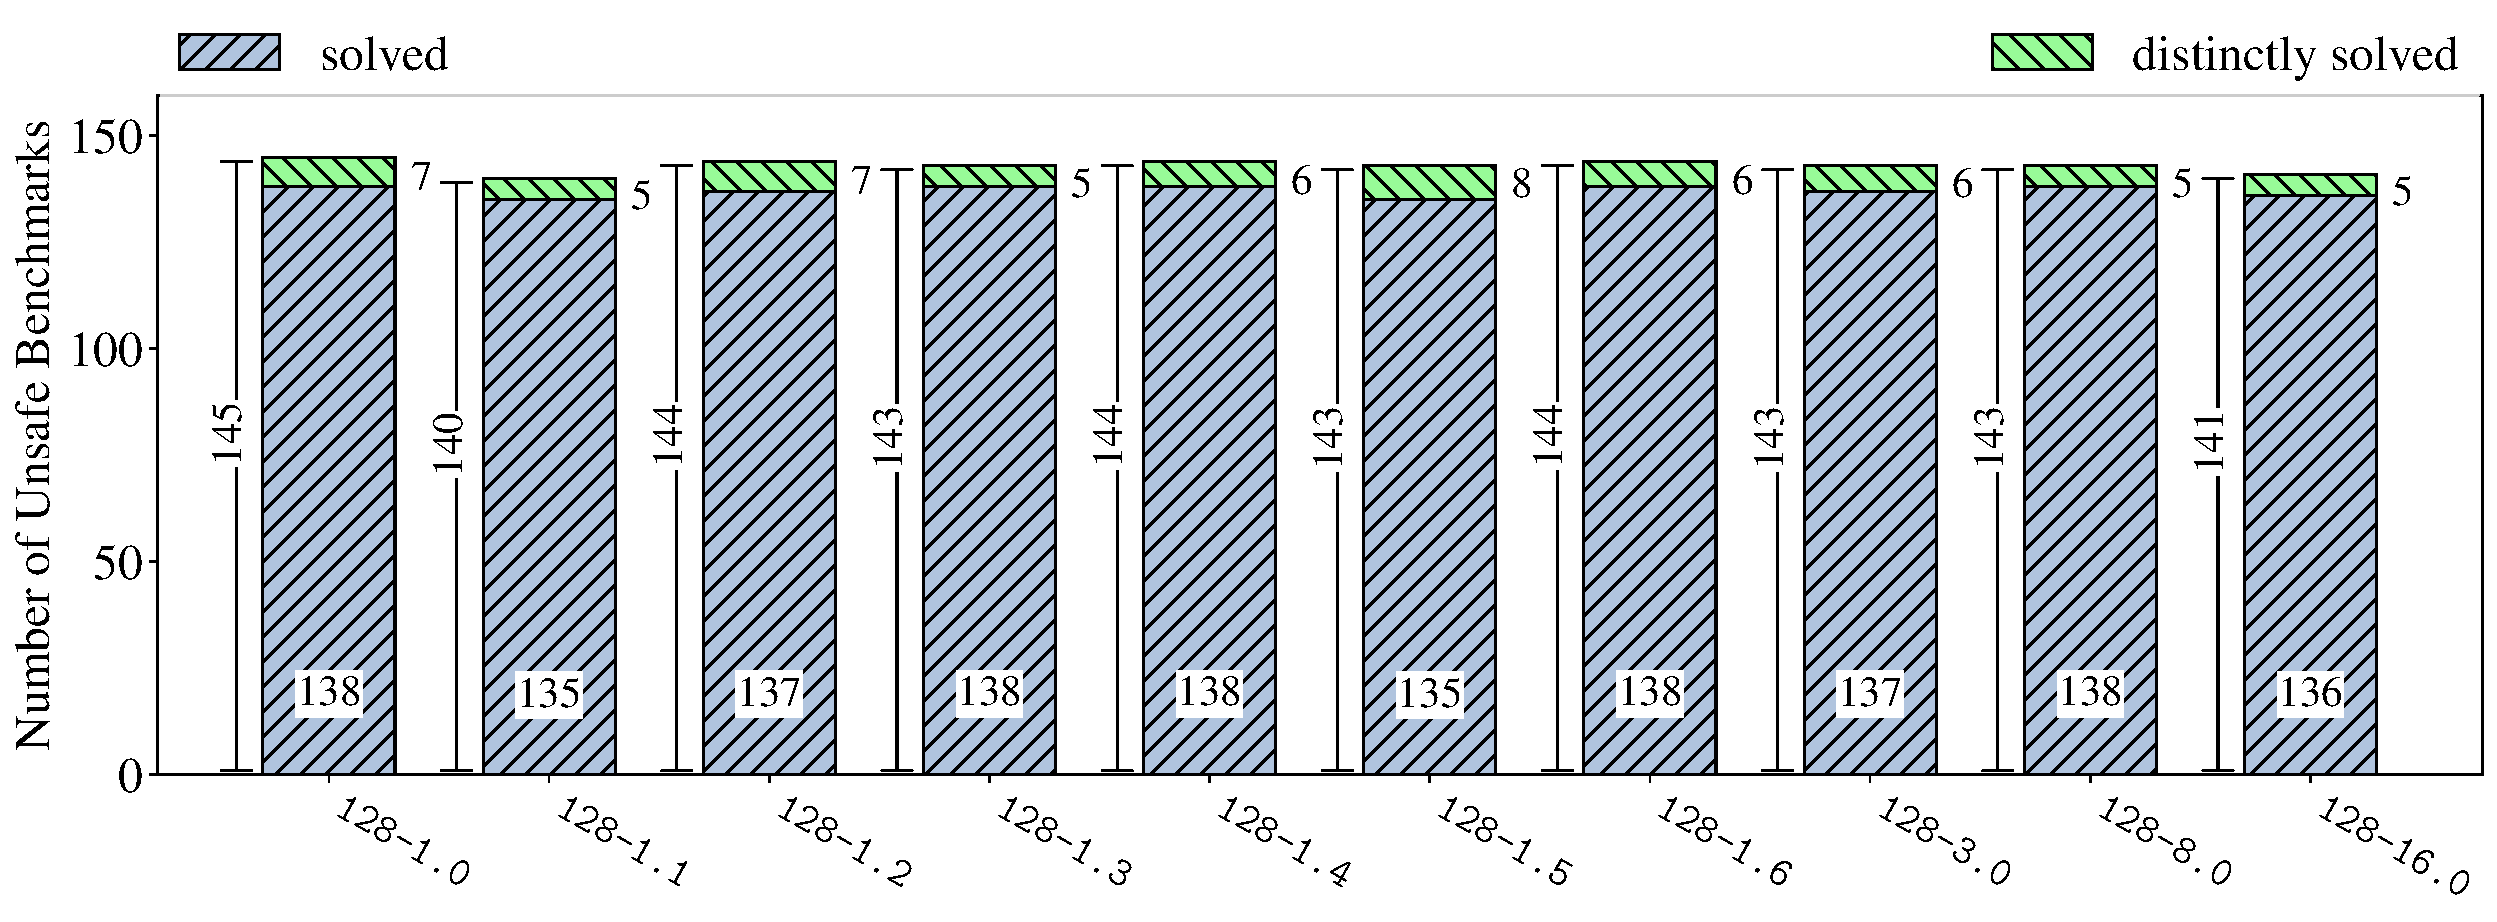
\includegraphics[width=0.98\linewidth]{images/128.pdf} \label{fig:car:128}
}
\subfigure[Implements of Restart Policy with $gr$ settled as $1.2$] { \label{fig:b} 
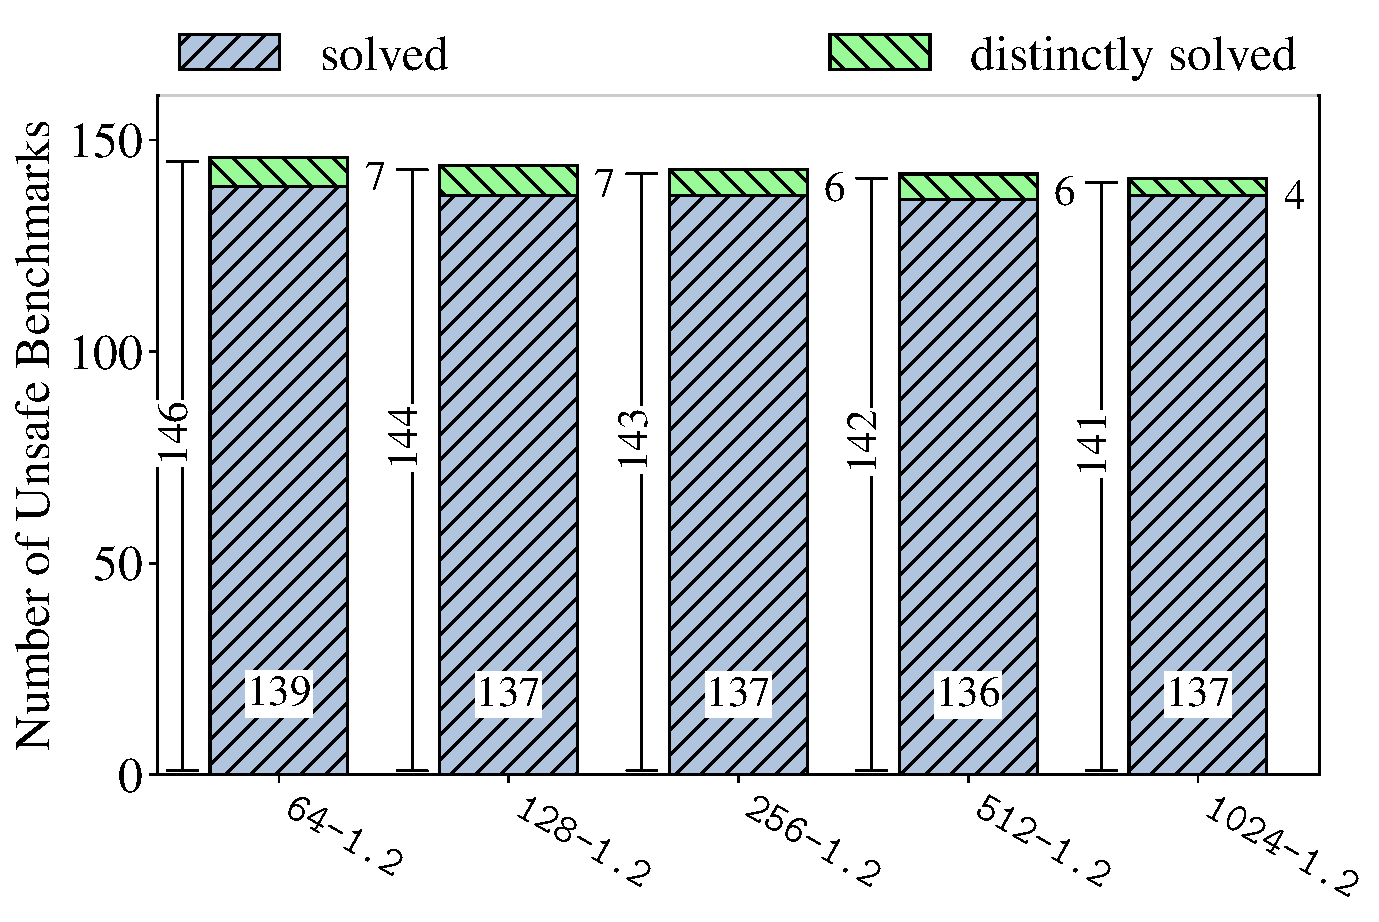
\includegraphics[width=0.49\linewidth]{images/1.2.pdf} \label{fig:car:1.2}
}
\subfigure[CAR vs. BMC] { \label{fig:c} 
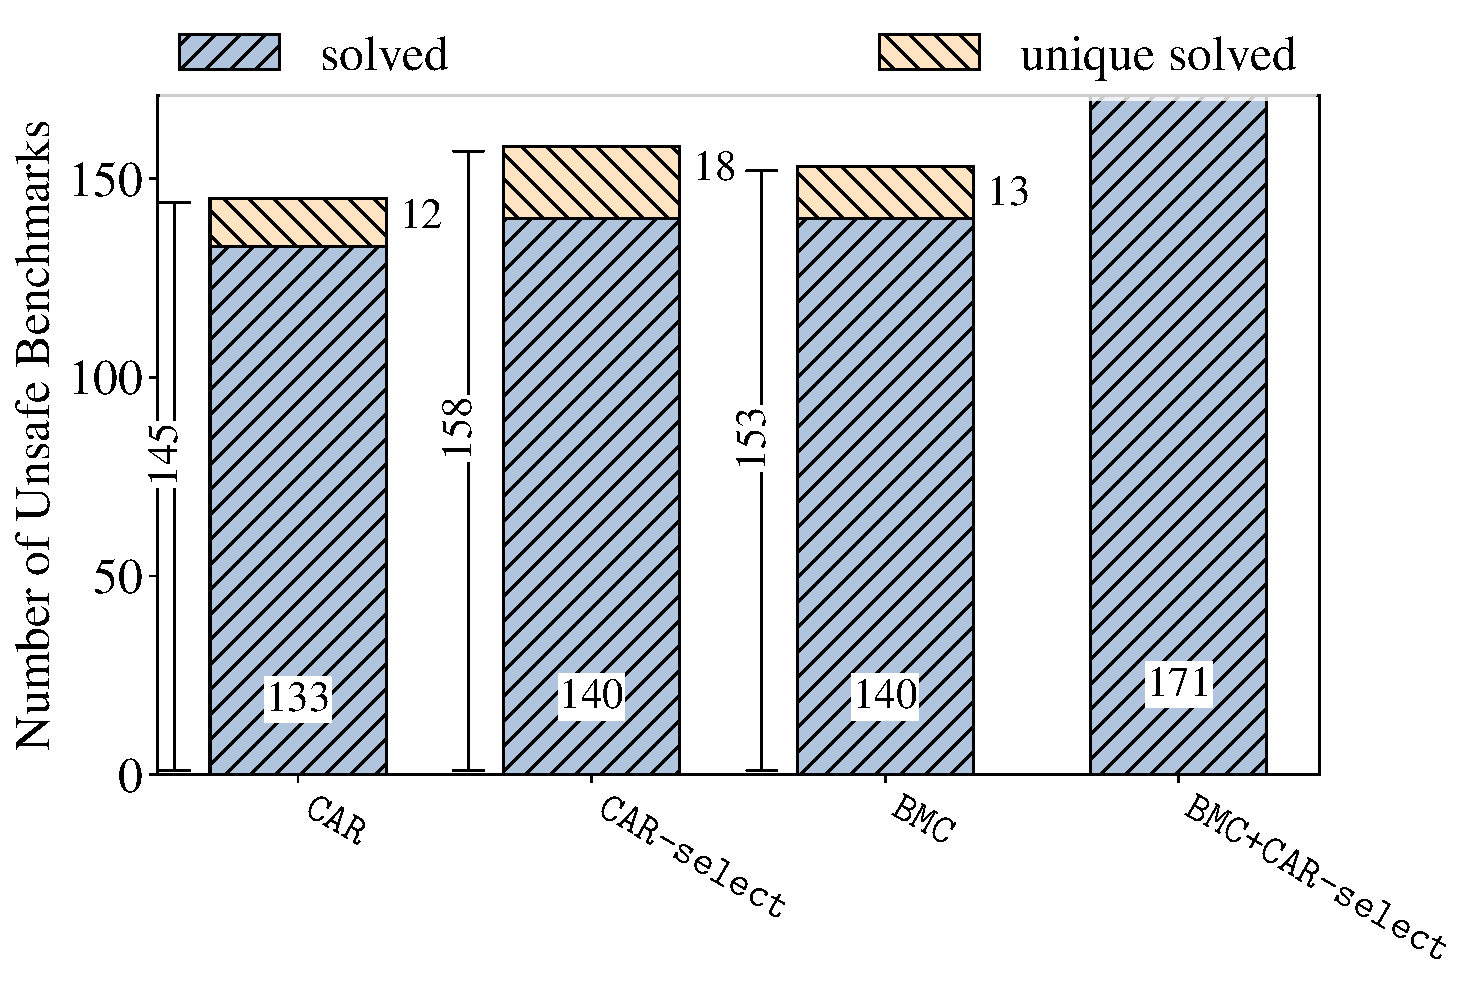
\includegraphics[width=0.49\linewidth]{images/car-bmc.pdf} \label{fig:compare}
}
\caption{Number of unsafe benchmarks solved by CAR after applying the restart policy. The category ``distinctly solved'' benchmarks are solved by CAR with the corresponding restart policy but not by the original CAR. The ``solved'' benchmarks solved by CAR with and without the restart policy. X-axis 128-1.0 means $threshold=128$, $gr=1.0$ and the same applies to others.}\label{fig:car}
\end{figure*}
\subsection{Experimental Setup}
We implement the restart policy to the SimpleCAR model checker \cite{simplecar}. As mentioned before, the restart frequency has a significant influence on the effectiveness of the restart policy. In our conjecture, the frequent restarts in CAR may not preserve the advantages already achieved, while a low frequency of the algorithm cannot help solve new instances. In our proposed algorithm, two parameters $threshold$ and $gr$ are introduced to determine the restart frequency in a dynamic way. We evaluate different combinations of these two parameters. We assign a relatively small value to $threshold$ and assign $gr$ a value equal to or greater than 1 to $gr$, i.e., $threshold = 128, gr = 1.2$, aiming to avoid the disadvantage of frequent restarts by gradually increasing the threshold after each restart. 

We compare our results to those from the original CAR implemented in SimpleCAR, as well as from BMC that is integrated in ABC tool \cite{BM10}, which is a prestigious model checker in the community and won the hardware model checking competition many times. Notably, there are kinds of BMC implementations in ABC, and we select the \emph{bmc2} which has the better performance based on previous evaluations \cite{LDPRV18}. Both SimpleCAR and ABC use the Minisat SAT solver \cite{minisat,ES04} as the computation engine for model checking. 

All the experiments are performed on a cluster consisting of 2304 processor cores in 192 nodes running REDHat 6.0 with a 2.83GHz CPU and 48GB of memory (RAM). In the experiments, the time limit is set to be one hour and the memory-use is 8 GB, for each instance.
We evaluate all algorithms against 749 industrial benchmarks from the single safety property track (SINGLE) of the HWMCC in 2015 \cite{hwmcc15} and 2017 \cite{hwmcc17}. Each instance in the benchmark is an aiger model, which formalizes the And-Invertor Graph \cite{aiger} of a circuit together with the safety property to be verified. 

This paper focuses on unsafe checking, under which a counterexample can be output to help identify the property violation. We use the aigsim tool from the Aiger package \cite{aigertools} to check whether the produced counterexamples are correct. We report that all the counterexamples generated from all checkers pass the test from aigsim.

\subsection{Results}

\subsubsection{Comparison to original CAR}
In the experiments, the original CAR is able to solve 145 unsafe instances without counterexamples.
To evaluate the performance of the restart policy on CAR from this paper, we first fix $threshold$ to be $128$ and make the growth rate $gr$ vary from 1.0 to 16.0. The number of solved and \emph{distinctively solved} (The meaning see the figure.) instances with the corresponding parameters are shown in Fig. \ref{fig:car:128}. From the figure, the restart policy effectively expands the algorithm's diversity by finding considerable new counterexamples with different configurations. In particular, the restart strategy has better results when $gr$ are set to be in $1 < gr < 2$, which are able to gain the most new instances (7 or 8). 


We then vary $threshold$ from 64 to 1024 by fixing $gr$ to be 1.0, 1.2 and 1.5 respectively. The results of setting $gr=1.2$ are shown in 
Fig. \ref{fig:car:1.2}. Observing the results from Fig. \ref{fig:car:1.2}, the restart policy performs the best when the value of $threshold$ is around 128, under which not only more ``distinctly solved'', but also several unique instances are detected. For example, ``oski15a08b15s'' can only be found by ``64-1.2'', ``6s351rb15'' can only be solved by ``128-1.2'' and ``oc8051topo08'' can only be solved by ``128-1.5''. Probably, some instances are sensitive to a particular combo of parameters, which determines the frequency of restart policy. Setting $threshold$ to the value 1024 seems to be too large for a one-hour experiment to make the restart strategy work. 

It should be highlighted that, although IC3/PDR can also perform differently by varying the paremeters to generate the inductive clauses \cite{GR16}, it help more to prove safe instances. Meanwhile, applying the restart policy to CAR results in a better performance on solving unsafe instances that can produce the counterexamples. 

\subsubsection{Comparison to original CAR and BMC }
As shown in Fig. \ref{fig:compare}, the BMC implementation in ABC solve 153 unsafe instances. We combined the results of five experiments(``64-1.2'', ``128-1.2'', ``128-1.5'', ``128-3.0'' and ``256-1.2'')and CAR, noted as ``CAR-select''. Observing ``'CAR-select'', the restart policy helps CAR find 13 more counterexamples (from 145 to 158) and 6 more ``unique solved''(from 12 to 18) that can only solved by CAR. Also, ``CAR-select'' solves 158 instances in total, which outperforms BMC (the amount is 153) and gains 18 instances that can not be found by BMC. The virtual combination of ``CAR-select'' and BMC solves 171 instances, which affirms that the restart policy plays a non-negligible role as a part of the portfolio for hardware model checking.

\section{Concluding Remarks}
In this paper, we apply the restart policy to Hardware Model Checking, aiming to get rid of the trap, which occurs during search and make the algorithm not terminate in a reasonable time. The results of the experiments show that the restart policy increases the diversity of the CAR algorithm, though there is no single configuration that can improve the overall performance significantly. The new finding of 13 unsafe instances indicates the efficiency of the restart policy in the domain. Moreover, the CAR algorithm with the restart policy can now find 18 unsafe instances with counterexamples that the BMC can not find, which enhances the ability of the current hardware model checking portfolio. 

This is the first work to understand how the restart policy performs on hardware model checking.
In future work, we plan to design more elaborate and sophisticated restart mechanisms to improve the overall performance of CAR such that it is able to outperform BMC on bug-finding with a single restart configuration. Due to the fact that different problems are sensitive to different restart frequencies, it is also interesting to introduce the learning techniques to learn a best solution for different instances. 


\iffalse
\begin{thebibliography}{00}
\bibitem{b1} Biere, A., Cimatti, A., Clarke, E., Zhu, Y.: Symbolic model checking without BDDs. In: Cleaveland, W.R. (ed.) Tools and Algorithms for the Construction and Analysis of Systems. pp. 193–207. Springer Berlin Heidelberg, Berlin, Heidelberg (1999)

\bibitem{b2} Li, J., Zhu, S., Zhang, Y., Pu, G., Vardi, M.Y.: Safety model checking with complementary approximations. In: Proceedings of the 36th International Conference on Computer-Aided Design, 2017, pp. 95–100

\bibitem{b3} Li, Jianwen, et al. "Simplecar: An efficient bug-finding tool based on approximate reachability." International Conference on Computer Aided Verification. Springer, Cham, 2018.

\bibitem{b4} Huang, Jinbo. "The Effect of Restarts on the Efficiency of Clause Learning." IJCAI. Vol. 7. 2007.

\bibitem{b5} Audemard, Gilles, and Laurent Simon. "Refining restarts strategies for SAT and UNSAT." International Conference on Principles and Practice of Constraint Programming. Springer, Berlin, Heidelberg, 2012.

\bibitem{b6} Een, N., Mishchenko, A., Brayton, R.: Efficient implementation of property directed reachability. In: Proceedings of the International Conference on Formal Methods in ComputerAided Design. pp. 125–134. FMCAD ’11, FMCAD Inc, Austin, TX (2011), http://dl. acm.org/citation.cfm?id=2157654.2157675

\bibitem{b7} Bradley, A.R.: Sat-based model checking without unrolling. In: Jhala, R., Schmidt, D. (eds.) Verification, Model Checking, and Abstract Interpretation. pp. 70–87. Springer Berlin Heidelberg, Berlin, Heidelberg (2011)

\bibitem{b8} McMillan, K.L.: Interpolation and sat-based model checking. In: Hunt, W.A., Somenzi, F. (eds.) Computer Aided Verification. pp. 1–13. Springer Berlin Heidelberg, Berlin, Heidelberg (2003)

\bibitem{b9} Biere, A., Cimatti, A., Clarke, E.M., Fujita, M., Zhu, Y.: Symbolic model checking using sat procedures instead of bdds (1999), http://doi.acm.org/10.1145/309847.309942

\bibitem{b10} HWMCC 2015. http://fmv.jku.at/hwmcc15/

\bibitem{b11} HWMCC 2017. http://fmv.jku.at/hwmcc17/

\bibitem{b12} Brayton, Robert, and Alan Mishchenko. "ABC: An academic industrial-strength verification tool." International Conference on Computer Aided Verification. Springer, Berlin, Heidelberg, 2010.
\end{thebibliography}
\fi



\UseRawInputEncoding
\tiny
\bibliographystyle{ieeetr}
\bibliography{dac.bib,cav.bib,ok.bib}







\iffalse
\section{Prepare Your Paper Before Styling}
Before you begin to format your paper, first write and save the content as a 
separate text file. Complete all content and organizational editing before 
formatting. Please note sections \ref{AA}--\ref{SCM} below for more information on 
proofreading, spelling and grammar.

Keep your text and graphic files separate until after the text has been 
formatted and styled. Do not number text heads---{\LaTeX} will do that 
for you.

\subsection{Abbreviations and Acronyms}\label{AA}
Define abbreviations and acronyms the first time they are used in the text, 
even after they have been defined in the abstract. Abbreviations such as 
IEEE, SI, MKS, CGS, ac, dc, and rms do not have to be defined. Do not use 
abbreviations in the title or heads unless they are unavoidable.

\subsection{Units}
\begin{itemize}
\item Use either SI (MKS) or CGS as primary units. (SI units are encouraged.) English units may be used as secondary units (in parentheses). An exception would be the use of English units as identifiers in trade, such as ``3.5-inch disk drive''.
\item Avoid combining SI and CGS units, such as current in amperes and magnetic field in oersteds. This often leads to confusion because equations do not balance dimensionally. If you must use mixed units, clearly state the units for each quantity that you use in an equation.
\item Do not mix complete spellings and abbreviations of units: ``Wb/m\textsuperscript{2}'' or ``webers per square meter'', not ``webers/m\textsuperscript{2}''. Spell out units when they appear in text: ``. . . a few henries'', not ``. . . a few H''.
\item Use a zero before decimal points: ``0.25'', not ``.25''. Use ``cm\textsuperscript{3}'', not ``cc''.)
\end{itemize}

\subsection{Equations}
Number equations consecutively. To make your 
equations more compact, you may use the solidus (~/~), the exp function, or 
appropriate exponents. Italicize Roman symbols for quantities and variables, 
but not Greek symbols. Use a long dash rather than a hyphen for a minus 
sign. Punctuate equations with commas or periods when they are part of a 
sentence, as in:
\begin{equation}
a+b=\gamma\label{eq}
\end{equation}

Be sure that the 
symbols in your equation have been defined before or immediately following 
the equation. Use ``\eqref{eq}'', not ``Eq.~\eqref{eq}'' or ``equation \eqref{eq}'', except at 
the beginning of a sentence: ``Equation \eqref{eq} is . . .''

\subsection{\LaTeX-Specific Advice}

Please use ``soft'' (e.g., \verb|\eqref{Eq}|) cross references instead
of ``hard'' references (e.g., \verb|(1)|). That will make it possible
to combine sections, add equations, or change the order of figures or
citations without having to go through the file line by line.

Please don't use the \verb|{eqnarray}| equation environment. Use
\verb|{align}| or \verb|{IEEEeqnarray}| instead. The \verb|{eqnarray}|
environment leaves unsightly spaces around relation symbols.

Please note that the \verb|{subequations}| environment in {\LaTeX}
will increment the main equation counter even when there are no
equation numbers displayed. If you forget that, you might write an
article in which the equation numbers skip from (17) to (20), causing
the copy editors to wonder if you've discovered a new method of
counting.

{\BibTeX} does not work by magic. It doesn't get the bibliographic
data from thin air but from .bib files. If you use {\BibTeX} to produce a
bibliography you must send the .bib files. 

{\LaTeX} can't read your mind. If you assign the same label to a
subsubsection and a table, you might find that Table I has been cross
referenced as Table IV-B3. 

{\LaTeX} does not have precognitive abilities. If you put a
\verb|\label| command before the command that updates the counter it's
supposed to be using, the label will pick up the last counter to be
cross referenced instead. In particular, a \verb|\label| command
should not go before the caption of a figure or a table.

Do not use \verb|\nonumber| inside the \verb|{array}| environment. It
will not stop equation numbers inside \verb|{array}| (there won't be
any anyway) and it might stop a wanted equation number in the
surrounding equation.

\subsection{Some Common Mistakes}\label{SCM}
\begin{itemize}
\item The word ``data'' is plural, not singular.
\item The subscript for the permeability of vacuum $\mu_{0}$, and other common scientific constants, is zero with subscript formatting, not a lowercase letter ``o''.
\item In American English, commas, semicolons, periods, question and exclamation marks are located within quotation marks only when a complete thought or name is cited, such as a title or full quotation. When quotation marks are used, instead of a bold or italic typeface, to highlight a word or phrase, punctuation should appear outside of the quotation marks. A parenthetical phrase or statement at the end of a sentence is punctuated outside of the closing parenthesis (like this). (A parenthetical sentence is punctuated within the parentheses.)
\item A graph within a graph is an ``inset'', not an ``insert''. The word alternatively is preferred to the word ``alternately'' (unless you really mean something that alternates).
\item Do not use the word ``essentially'' to mean ``approximately'' or ``effectively''.
\item In your paper title, if the words ``that uses'' can accurately replace the word ``using'', capitalize the ``u''; if not, keep using lower-cased.
\item Be aware of the different meanings of the homophones ``affect'' and ``effect'', ``complement'' and ``compliment'', ``discreet'' and ``discrete'', ``principal'' and ``principle''.
\item Do not confuse ``imply'' and ``infer''.
\item The prefix ``non'' is not a word; it should be joined to the word it modifies, usually without a hyphen.
\item There is no period after the ``et'' in the Latin abbreviation ``et al.''.
\item The abbreviation ``i.e.'' means ``that is'', and the abbreviation ``e.g.'' means ``for example''.
\end{itemize}
An excellent style manual for science writers is \cite{b7}.

\subsection{Authors and Affiliations}
\textbf{The class file is designed for, but not limited to, six authors.} A 
minimum of one author is required for all conference articles. Author names 
should be listed starting from left to right and then moving down to the 
next line. This is the author sequence that will be used in future citations 
and by indexing services. Names should not be listed in columns nor group by 
affiliation. Please keep your affiliations as succinct as possible (for 
example, do not differentiate among departments of the same organization).

\subsection{Identify the Headings}
Headings, or heads, are organizational devices that guide the reader through 
your paper. There are two types: component heads and text heads.

Component heads identify the different components of your paper and are not 
topically subordinate to each other. Examples include Acknowledgments and 
References and, for these, the correct style to use is ``Heading 5''. Use 
``figure caption'' for your Figure captions, and ``table head'' for your 
table title. Run-in heads, such as ``Abstract'', will require you to apply a 
style (in this case, italic) in addition to the style provided by the drop 
down menu to differentiate the head from the text.

Text heads organize the topics on a relational, hierarchical basis. For 
example, the paper title is the primary text head because all subsequent 
material relates and elaborates on this one topic. If there are two or more 
sub-topics, the next level head (uppercase Roman numerals) should be used 
and, conversely, if there are not at least two sub-topics, then no subheads 
should be introduced.

\subsection{Figures and Tables}
\paragraph{Positioning Figures and Tables} Place figures and tables at the top and 
bottom of columns. Avoid placing them in the middle of columns. Large 
figures and tables may span across both columns. Figure captions should be 
below the figures; table heads should appear above the tables. Insert 
figures and tables after they are cited in the text. Use the abbreviation 
``Fig.~\ref{fig}'', even at the beginning of a sentence.

\begin{table}[htbp]
\caption{Table Type Styles}
\begin{center}
\begin{tabular}{|c|c|c|c|}
\hline
\textbf{Table}&\multicolumn{3}{|c|}{\textbf{Table Column Head}} \\
\cline{2-4} 
\textbf{Head} & \textbf{\textit{Table column subhead}}& \textbf{\textit{Subhead}}& \textbf{\textit{Subhead}} \\
\hline
copy& More table copy$^{\mathrm{a}}$& &  \\
\hline
\multicolumn{4}{l}{$^{\mathrm{a}}$Sample of a Table footnote.}
\end{tabular}
\label{tab1}
\end{center}
\end{table}

\begin{figure}[htbp]
\centerline{
\includegraphics{fig1.png}}
\caption{Example of a figure caption.}
\label{fig}
\end{figure}

Figure Labels: Use 8 point Times New Roman for Figure labels. Use words 
rather than symbols or abbreviations when writing Figure axis labels to 
avoid confusing the reader. As an example, write the quantity 
``Magnetization'', or ``Magnetization, M'', not just ``M''. If including 
units in the label, present them within parentheses. Do not label axes only 
with units. In the example, write ``Magnetization (A/m)'' or ``Magnetization 
\{A[m(1)]\}'', not just ``A/m''. Do not label axes with a ratio of 
quantities and units. For example, write ``Temperature (K)'', not 
``Temperature/K''.

\section*{Acknowledgment}

The preferred spelling of the word ``acknowledgment'' in America is without 
an ``e'' after the ``g''. Avoid the stilted expression ``one of us (R. B. 
G.) thanks $\ldots$''. Instead, try ``R. B. G. thanks$\ldots$''. Put sponsor 
acknowledgments in the unnumbered footnote on the first page.

\section*{References}

Please number citations consecutively within brackets \cite{b1}. The 
sentence punctuation follows the bracket \cite{b2}. Refer simply to the reference 
number, as in \cite{b3}---do not use ``Ref. \cite{b3}'' or ``reference \cite{b3}'' except at 
the beginning of a sentence: ``Reference \cite{b3} was the first $\ldots$''

Number footnotes separately in superscripts. Place the actual footnote at 
the bottom of the column in which it was cited. Do not put footnotes in the 
abstract or reference list. Use letters for table footnotes.

Unless there are six authors or more give all authors' names; do not use 
``et al.''. Papers that have not been published, even if they have been 
submitted for publication, should be cited as ``unpublished'' \cite{b4}. Papers 
that have been accepted for publication should be cited as ``in press'' \cite{b5}. 
Capitalize only the first word in a paper title, except for proper nouns and 
element symbols.

For papers published in translation journals, please give the English 
citation first, followed by the original foreign-language citation \cite{b6}.

\begin{thebibliography}{00}
\bibitem{b1} G. Eason, B. Noble, and I. N. Sneddon, ``On certain integrals of Lipschitz-Hankel type involving products of Bessel functions,'' Phil. Trans. Roy. Soc. London, vol. A247, pp. 529--551, April 1955.
\bibitem{b2} J. Clerk Maxwell, A Treatise on Electricity and Magnetism, 3rd ed., vol. 2. Oxford: Clarendon, 1892, pp.68--73.
\bibitem{b3} I. S. Jacobs and C. P. Bean, ``Fine particles, thin films and exchange anisotropy,'' in Magnetism, vol. III, G. T. Rado and H. Suhl, Eds. New York: Academic, 1963, pp. 271--350.
\bibitem{b4} K. Elissa, ``Title of paper if known,'' unpublished.
\bibitem{b5} R. Nicole, ``Title of paper with only first word capitalized,'' J. Name Stand. Abbrev., in press.
\bibitem{b6} Y. Yorozu, M. Hirano, K. Oka, and Y. Tagawa, ``Electron spectroscopy studies on magneto-optical media and plastic substrate interface,'' IEEE Transl. J. Magn. Japan, vol. 2, pp. 740--741, August 1987 [Digests 9th Annual Conf. Magnetics Japan, p. 301, 1982].
\bibitem{b7} M. Young, The Technical Writer's Handbook. Mill Valley, CA: University Science, 1989.
\end{thebibliography}
\vspace{12pt}
\color{red}
IEEE conference templates contain guidance text for composing and formatting conference papers. Please ensure that all template text is removed from your conference paper prior to submission to the conference. Failure to remove the template text from your paper may result in your paper not being published.

\fi

\end{document}
